% ***************************************** SYMBOLS
\def\abs#1{\lvert#1\rvert}
\def\argdot{{\hspace{0.18em}\cdot\hspace{0.18em}}}
\def\avg#1{\left\{#1\right\}_\omega}
\def\D{{\tn D}}
\def\div{\operatorname{div}}
\def\Eh{\mathcal E_h}       % edges of \Th
\def\Ehcom{\mathcal E_{h,C}}         % edges of \Th on interface with lower dimension
\def\Ehdir{\mathcal E_{h,D}}         % Dirichlet edges of \Th
\def\Ehint{\mathcal E_{h,I}}       % interior edges of \Th
\def\grad{\nabla}
\def\jmp#1{[#1]}
\def\n{\vc n}
\def\vc#1{\mathbf{\boldsymbol{#1}}}     % vector
\def\R{\mathbb R}
\def\sc#1#2{\left(#1,#2\right)}
\def\Th{\mathcal T_h}       % triangulation
\def\th{\vartheta}
\def\tn#1{{\mathbb{#1}}}    % tensor
\def\Tr{\operatorname{Tr}}
\def\where{\,|\,}
%***************************************************************************

\section{Equilibrial Adsorption}\label{sec:sorp_math}
The simulation of monolayer, equilibrial adsorption is based on solution of the couple of equations representing mass balance law and empirical description of adsorption represented by common types of isotherm. The following types of isotherm are considered:
\begin{itemize}
 \item Without adsorption, \hyperA{Sorption-BulkData::sorption-types}{$sorption\_type$} is ``$none$''.
 \item Linear isotherm $c_s = f(c_a) = k_l\cdot c_a$, $sorption\_type$ is ``$linear$''.
 \item Freundlichs' isotherm $c_s = f(c_a) = k_F\cdot c_a^{\alpha}$, $sorption\_type$ is ``$freundlich$''.
 \item Langmuirs' isotherm $c_s = f(c_a) = k_L\cdot \frac{\alpha\cdot c_a}{1 + \alpha\cdot c_a}$, $sorption\_type$ is ``$langmuir$''. Langmuirs isotherm has been derived from thermodynamic laws. $k_L$ denotes the maximal amount of sorbing specie which can be kept in an unit volume of a bulk matrix. Coefficient $\alpha$ is a fraction of adsorption and desorption rate constant $\alpha = \frac{k_a}{k_d}$.
\end{itemize}
Notification:
\begin{itemize}
 \item Sorbed concentration $[c_s] = \frac{[n]}{[m_H]} = \frac{N}{M} = \frac{Mol}{kg}$, where $m_H$ is the mass of bulk and $n$ denotes amount of substance in an element.
 \item Aqueous concentration $[c_a] = \frac{[m]}{[m_w]} = \frac{M}{M} = \frac{kg}{kg} = 1$, where $m_w$ is the mass of water/solvent in an element. Just water ($\rho_w = 1~kg\cdot l^{-1}$) is supposed to be solvent in version 1.7.0. 
 \item Multiplication parameters, $k_i, ~i\in\{ l,F,L\}$, \hyperA{Sorption-BulkData::mult-coefs}{$mult\_coefs$} can have various physical dimensions.
 \item Additional parameters, $[\alpha] = 1$, \hyperA{Sorption-BulkData::second-params}{$second\_params$}.
\end{itemize}
The mass balance equation can be derived from \ref{eq:mass_balance_base},
\begin{equation}
  m_{Total} = m_{aqueous} + m_{sorbed} = c_a\cdot V_{elm}\cdot\rho_w\cdot n + c_s\cdot M_s \cdot V_{elm}\cdot\rho_H\cdot(1-n)
  \label{eq:mass_balance_base}
\end{equation}
where $\rho_w$ denotes solvent density \hyperA{Sorptions::solvent-dens}{$solvent\_dens$}, $\rho_H$ is the symbol for \hyperA{Sorption-BulkData::rock-density}{$rock\_density$}, $V_{elm}$ denotes element volume, $n$ is the symbol for porosity, here, and $M_s$ denotes \hyperA{Sorptions::molar-masses}{$molar\_masses$}.

The equation \ref{eq:mass_balance_base} depends on volume of an element $V_{elm}$. We devide both sides by $V_{elm}$ to suppress this dependency and we get resulting mass balance equation \ref{eq:mass_balance_base2}.
\begin{equation}
 \begin{array}{l}
  konst._T = k_a\cdot c_a + k_s\cdot c_s\\
  k_a = \rho_w\cdot n\\
  k_s = M_s \cdot\rho_H\cdot(1-n)
 \end{array}
 \label{eq:mass_balance_base2}
\end{equation}

After the substitution $|c_s = f(c_a)|$ we obtain the equation, which can be either solved iteratively or aproximated through interpolation. This equation has following form.
\begin{equation}
 konst._T = k_a\cdot c_a + k_s\cdot f(c_a)
 \label{eq:nonlin_sorption}
\end{equation}
To solve the equation \ref{eq:nonlin_sorption} iteratively, it is very important to define interval where to look for solution (unknown $c_a$). The lower bound is $0$. Concentration can not reach negative values. The upper bound is derived using simple imagination. Lets suppose limmited \hyperA{Sorptions::solubility}{$solubility$} of selected transported substance and lets denote the limmit $c_a^{limmit}$. We keep the maximal "total mass" $konst._T^{limit}= k_a\cdot c_a^{limmit} + k_s\cdot f(c_a^{limmit})$, but we dissolve all the mass to get maximal $c_a^{max} > c_a^{limmit}$. That means $c_s = 0$ for this moment. To understand this step lets look at the figure \ref{fig:sorpce}. We can slightly enlarge the interval by setting the upper bound equal to $c_a^{max} + const_{small}$.

\begin{figure}[ht!]
 \centering
 \includegraphics[scale = 1.0]{\fig/sorpce}
 \caption{Sorption in combination with limmited solubility.}
 \label{fig:sorpce}
\end{figure}


To approximate the equation \ref{eq:nonlin_sorption} using interpolation we need to prepare the set of values which represent $[c_a, f(c_a)]$, with $c_a$ equidistantly distributed in transformed (rotated and rescaled) coordination system at first. The approach for construction of interpolation table follows.
\begin{enumerate}
 \item Maximal "total mass" $konst._T^{limit} = k_a\cdot c_a^{limmit} + k_s\cdot f(c_a^{limmit})$ is computed.
 \item Total mass step is derived $mass\_step = konst._T^{limit}/n\_steps$. $n\_steps$ is equal to \hyperA{Sorptions::substeps}{$substeps$} in con-file.
 \item Appropriate $c_a^i = (mass\_step\cdot i)/k_a,~i\in \{0,\ldots, n\_steps\}$ are computed. 
 \item The equations $k_a\cdot c_a^i = k_a\cdot c_a + k_s\cdot f(c_a)~i\in \{0,\ldots, n\_steps\}$ are solved for $c_a$ as unknown. The solution is the set of ordered couples (points) $[c_a^l,f(c_a^l)],~l\in\{0,\ldots,n\_steps\}$.
\end{enumerate}
After computation of $\{[c_a^l,f(c_a^l)]\}$ we transform these coordinates to the system where total mass is independent variable. This is done by multiplication of precomputed points using transformation matrix ${\bf A}$.
\begin{equation}
 \begin{array}{l}
  \overrightarrow{c}^R = {\bf A}\cdot\overrightarrow{c}\\
  \left[\begin{array}{c} c_a^{R,l}\\ c_s^{R,l} \end{array}\right] = 
  \left[\begin{array}{cc}
    n\cdot \rho_w & M_s(1 - n)\rho_H\\
    -M_s(1 - n)\rho_H & n\cdot \rho_w
  \end{array}\right]\cdot
  \left[\begin{array}{c} c_a^l\\ c_s^l \end{array}\right]\\
  l\in\{0,\ldots,n\_steps\}
 \end{array}
 \label{eq:transf_mat}
\end{equation}

The values $c_a^{R,l}$ are equidistantly distributed and there is no reason to save them, but the values $c_s^{R,l}$ are stored in onedimensional interpolation table.

Once we have the interpolation table, we can use it for projection of ${[c_a,c_s]}$ transport results on the isotherm under concideration. The approach look as folows.
\begin{enumerate}
 \item Achieved concentrations are transformed to the coordination system through multiplication with the matrix ${\bf A}$, see \ref{eq:transf_mat}.
 \item Transrformed values are interpolated.
 \item The result of interpolation is transformed back. The backward transformation consist of multiplication with ${\bf A}^T$ which is followed by rescaling the result. Rescaling the result is neccessery because  ${\bf A}$ is not orthonormal as it is shown bellow.
 \[
 \begin{array}{l}
 {\bf A}^T\cdot{\bf A} =
  \left((n - 1)^2\cdot M_s^2\cdot \rho_h^2 + n^2\cdot \rho_w^2\right)\cdot\left[\begin{array}{cc}
    1 & 0\\
    0 & 1
  \end{array}\right]
  \end{array}
 \]
\end{enumerate}


\subsection{Limmited Solubility}\label{subsec:lim_solub}
When $k_a\cdot c_a + k_s\cdot f(c_a) > k_a\cdot c_a^{limmit} + k_s\cdot f(c_a^{limmit})$ neither iterative solver nor interpolation table is used. The aqueous concentration is set to be $c_a^{limmit}$ and sorbed concentration is computed $c_s = (k_a\cdot c_a + k_s\cdot f(c_a) - k_a\cdot c_a^{limmit})/k_s$.